\iffalse
This file is protected by Copyright. Please refer to the COPYRIGHT file
distributed with this source distribution.

This file is part of OpenCPI <http://www.opencpi.org>

OpenCPI is free software: you can redistribute it and/or modify it under the
terms of the GNU Lesser General Public License as published by the Free Software
Foundation, either version 3 of the License, or (at your option) any later
version.

OpenCPI is distributed in the hope that it will be useful, but WITHOUT ANY
WARRANTY; without even the implied warranty of MERCHANTABILITY or FITNESS FOR A
PARTICULAR PURPOSE. See the GNU Lesser General Public License for more details.

You should have received a copy of the GNU Lesser General Public License along
with this program. If not, see <http://www.gnu.org/licenses/>.
\fi

%----------------------------------------------------------------------------------------
% Update the docTitle and docVersion per document
%----------------------------------------------------------------------------------------
\def\docTitle{OpenCPI\\ FSK App Getting Started Guide\\ (E310 Supplement)}
\def\docVersion{1.5}
%----------------------------------------------------------------------------------------
\documentclass{article}
\iffalse
This file is protected by Copyright. Please refer to the COPYRIGHT file
distributed with this source distribution.

This file is part of OpenCPI <http://www.opencpi.org>

OpenCPI is free software: you can redistribute it and/or modify it under the
terms of the GNU Lesser General Public License as published by the Free Software
Foundation, either version 3 of the License, or (at your option) any later
version.

OpenCPI is distributed in the hope that it will be useful, but WITHOUT ANY
WARRANTY; without even the implied warranty of MERCHANTABILITY or FITNESS FOR A
PARTICULAR PURPOSE. See the GNU Lesser General Public License for more details.

You should have received a copy of the GNU Lesser General Public License along
with this program. If not, see <http://www.gnu.org/licenses/>.
\fi
% Any changes to this document should be made in opencpi.git
\author{} % Force author to be blank
%----------------------------------------------------------------------------------------
% Paper size, orientation and margins
%----------------------------------------------------------------------------------------
\usepackage{geometry}
\geometry{
        letterpaper, % paper type
        portrait,    % text direction
        left=.75in,  % left margin
        top=.75in,   % top margin
        right=.75in, % right margin
        bottom=.75in % bottom margin
 }
%----------------------------------------------------------------------------------------
% Header/Footer
%----------------------------------------------------------------------------------------
\usepackage{fancyhdr} \pagestyle{fancy} % required for fancy headers
\renewcommand{\headrulewidth}{0.5pt}
\renewcommand{\footrulewidth}{0.5pt}
\rhead{\small{ANGRYVIPER Team}}
% \rfoot{\thepage}
%----------------------------------------------------------------------------------------
% Appendix packages
%----------------------------------------------------------------------------------------
\usepackage[toc,page]{appendix}
%----------------------------------------------------------------------------------------
% Defined Commands & Renamed Commands
%----------------------------------------------------------------------------------------
\renewcommand{\contentsname}{Table of Contents}
\renewcommand{\listfigurename}{List of Figures}
\renewcommand{\listtablename}{List of Tables}
\newcommand{\todo}[1]{\textcolor{red}{TODO: #1}\PackageWarning{TODO:}{#1}} % To do notes
\newcommand{\code}[1]{\texttt{#1}} % For inline code snippet or command line
%----------------------------------------------------------------------------------------
% Various packages
%----------------------------------------------------------------------------------------
\usepackage[usenames,dvipsnames]{xcolor} % for color names see https://en.wikibooks.org/wiki/LaTeX/Colors
\usepackage{hyperref}  % for linking urls and lists
\usepackage{graphicx}  % for including pictures by file
\usepackage{listings}  % for coding language styles
\usepackage{rotating}  % for sideways table
\usepackage{pifont}    % for sideways table
\usepackage{pdflscape} % for landscape view
\usepackage{subfig}
\hyphenation{ANGRY-VIPER} % Tell it where to hyphenate
\hyphenation{Cent-OS} % Tell it where to hyphenate
\hyphenation{install-ation} % Tell it where to hyphenate
\uchyph=0 % Never hyphenate acronyms like RCC (I think this overrides ANGRYVIPER above)
\renewcommand\_{\textunderscore\allowbreak} % Allow words to break/newline on underscores
%----------------------------------------------------------------------------------------
% Table packages
%----------------------------------------------------------------------------------------
\usepackage{longtable} % for long possibly multi-page tables
\usepackage{tabularx} % c=center,l=left,r=right,X=fill
% These define tabularx columns "C" and "R" to match "X" but center/right aligned
\newcolumntype{C}{>{\centering\arraybackslash}X}
\newcolumntype{R}{>{\raggedleft\arraybackslash}X}
\usepackage{float}
\floatstyle{plaintop}
\usepackage[tableposition=top]{caption}
\newcolumntype{P}[1]{>{\centering\arraybackslash}p{#1}}
\newcolumntype{M}[1]{>{\centering\arraybackslash}m{#1}}
%----------------------------------------------------------------------------------------
% Block Diagram / FSM Drawings
%----------------------------------------------------------------------------------------
\usepackage{tikz}
\usetikzlibrary{shapes,arrows,fit,positioning}
\usetikzlibrary{automata} % used for the fsm
%----------------------------------------------------------------------------------------
% Colors Used
%----------------------------------------------------------------------------------------
\usepackage{colortbl}
\definecolor{blue}{rgb}{.7,.8,.9}
\definecolor{ceruleanblue}{rgb}{0.16, 0.32, 0.75}
\definecolor{drkgreen}{rgb}{0,0.6,0}
\definecolor{deepmagenta}{rgb}{0.8, 0.0, 0.8}
\definecolor{cyan}{rgb}{0.0,0.6,0.6}
\definecolor{maroon}{rgb}{0.5,0,0}
%----------------------------------------------------------------------------------------
% VHDL Coding Language Style
% modified from: http://latex-community.org/forum/viewtopic.php?f=44&t=22076
%----------------------------------------------------------------------------------------
\lstdefinelanguage{VHDL}
{
        basicstyle=\ttfamily\footnotesize,
        columns=fullflexible,keepspaces,      % https://tex.stackexchange.com/a/46695/87531
        keywordstyle=\color{ceruleanblue},
        commentstyle=\color{drkgreen},
        morekeywords={
    library,use,all,entity,is,port,in,out,end,architecture,of,
    begin,and, signal, when, if, else, process, end,
        },
        morecomment=[l]--
}
%----------------------------------------------------------------------------------------
% XML Coding Language Style
% modified from: http://tex.stackexchange.com/questions/10255/xml-syntax-highlighting
%----------------------------------------------------------------------------------------
\lstdefinelanguage{XML}
{
        basicstyle=\ttfamily\footnotesize,
        columns=fullflexible,keepspaces,
        morestring=[s]{"}{"},
        morecomment=[s]{!--}{--},
        commentstyle=\color{drkgreen},
        moredelim=[s][\color{black}]{>}{<},
        moredelim=[s][\color{cyan}]{\ }{=},
        stringstyle=\color{maroon},
        identifierstyle=\color{ceruleanblue}
}
%----------------------------------------------------------------------------------------
% DIFF Coding Language Style
% modified from http://tex.stackexchange.com/questions/50176/highlighting-a-diff-file
%----------------------------------------------------------------------------------------
\lstdefinelanguage{diff}
{
        basicstyle=\ttfamily\footnotesize,
        columns=fullflexible,keepspaces,
        breaklines=true,                                % wrap text
        morecomment=[f][\color{ceruleanblue}]{@@},      % group identifier
        morecomment=[f][\color{red}]-,                  % deleted lines
        morecomment=[f][\color{drkgreen}]+,             % added lines
        morecomment=[f][\color{deepmagenta}]{---},      % Diff header lines (must appear after +,-)
        morecomment=[f][\color{deepmagenta}]{+++},
}
%----------------------------------------------------------------------------------------
% Python Coding Language Style
% modified from
%----------------------------------------------------------------------------------------
\lstdefinelanguage{python}
{
        basicstyle=\ttfamily\footnotesize,
        columns=fullflexible,keepspaces,
        keywordstyle=\color{ceruleanblue},
        commentstyle=\color{drkgreen},
        stringstyle=\color{orange},
        morekeywords={
    print, if, sys, len, from, import, as, open,close, def, main, for, else, write, read, range,
        },
        comment=[l]{\#}
}
%----------------------------------------------------------------------------------------
% Fontsize Notes in order from smallest to largest
%----------------------------------------------------------------------------------------
%    \tiny
%    \scriptsize
%    \footnotesize
%    \small
%    \normalsize
%    \large
%    \Large
%    \LARGE
%    \huge
%    \Huge

\date{Version \docVersion} % Force date to be blank and override date with version
\title{\docTitle}
\lhead{FSK App Getting Started Guide}
%----------------------------------------------------------------------------------------
\usepackage[T1]{fontenc} % http://tex.stackexchange.com/a/181119
\usepackage{graphicx}
\graphicspath{ {figures/} }
\usepackage{textcomp}
\begin{document}
\maketitle
%\thispagestyle{fancy}
\newpage

	\begin{center}
	\textit{\textbf{Revision History}}
		\begin{table}[H]
		\label{table:revisions} % Add "[H]" to force placement of table
			\begin{tabularx}{\textwidth}{|c|X|l|}
			\hline
			\rowcolor{blue}
			\textbf{Revision} & \textbf{Description of Change} & \textbf{Date} \\
		    \hline
			v1.4 & Updated with simplifications and references to assets' document & 9/2018 \\
			\hline
			v1.5 & Version bump only & 4/2019 \\
			\hline
			\end{tabularx}
		\end{table}
	\end{center}

\newpage

\tableofcontents

\def\assetsdoc{\noindent For more information on this application, see \code{ocpi.assets}'s more in-depth version of the \textit{FSK\_app} document.}

\newpage

\section{References}

	This document assumes a basic understanding of the Linux command line (or ``shell'') environment.  The reference(s) in Table 1 can be used as an overview of OpenCPI and may prove useful.

\def\myreferences{
\hline
FSK App\footnote{Provides details of the ``FSK App'' reference application} & OpenCPI & \path{FSK_app.pdf}\\
}
\iffalse
This file is protected by Copyright. Please refer to the COPYRIGHT file
distributed with this source distribution.

This file is part of OpenCPI <http://www.opencpi.org>

OpenCPI is free software: you can redistribute it and/or modify it under the
terms of the GNU Lesser General Public License as published by the Free Software
Foundation, either version 3 of the License, or (at your option) any later
version.

OpenCPI is distributed in the hope that it will be useful, but WITHOUT ANY
WARRANTY; without even the implied warranty of MERCHANTABILITY or FITNESS FOR A
PARTICULAR PURPOSE. See the GNU Lesser General Public License for more details.

You should have received a copy of the GNU Lesser General Public License along
with this program. If not, see <http://www.gnu.org/licenses/>.
\fi

% This snippet creates the "References" table labeled "table:references"
% It creates three columns: Name, Publisher, Link and then inserts default documents
%
% To skip these defaults, define macros named
% refskipgs to skip "Getting Started"
% refskipig to skip "Installation Guide"
% refskipac to skip "Acronyms and Definitions"
% refskipocpiov to skip "OpenCPI Overview"
%
% See RPM_Installation_Guide.tex for examples
%
% After the defaults, it optionally inserts the "myreferences" macro that
% you defined elsewhere (you put hlines above all lines)
%
% If you want the \caption on the bottom, define "refcapbottom"
\begin{center}
\renewcommand*\footnoterule{} % Remove separator line from footnote
\renewcommand{\thempfootnote}{\arabic{mpfootnote}} % Use Arabic numbers (or can't reuse)
\begin{minipage}{0.9\textwidth}
  \begin{table}[H]
\ifx\refcapbottom\undefined
  \caption {References}
  \label{table:references}
\fi
  \begin{tabularx}{\textwidth}{|C|c|C|}
    \hline
    \rowcolor{blue}
    \textbf{Title} & \textbf{Published By} & \textbf{Link} \\
\ifx\refskipgs\undefined
    \hline
    Getting Started & ANGRYVIPER Team & \path{Getting_Started.pdf} \\
\fi
\ifx\refskipig\undefined
    \hline
    Installation Guide & ANGRYVIPER Team & \path{RPM_Installation_Guide.pdf} \\
\fi
\ifx\refskipac\undefined
    \hline
    Acronyms and Definitions & ANGRYVIPER Team & \path{Acronyms_and_Definitions.pdf} \\
\fi
\ifx\refskipocpiov\undefined
    \hline
    Overview & OpenCPI &
% Analytics: https://goo.gl/info/RskxiV
\url{https://goo.gl/RskxiV} \\
\fi
\ifx\myreferences\undefined
\else
    \myreferences
\fi
    \hline
  \end{tabularx}
\ifx\refcapbottom\undefined
\else
  \caption {References}
  \label{table:references}
\fi
  \end{table}
\end{minipage}
\end{center}


\newpage
\begin{flushleft}
\section{Overview}
The purpose of this document is to provide a compact set of instructions to build, run, and verify the OpenCPI FSK App reference application.

\section{Prerequisites}
This document assumes that the OpenCPI framework has been installed. The application is supported on the Ettus E310 platform.

\section{Build the OpenCPI Core Project}
If the Core Project has not been created yet, follow the instructions in the OpenCPI Getting Started Guide. Once the Core project has been created, the following ocpidev command can be used to build the primitives and workers required by the FSK app. Run the following:
\lstset{language=bash, backgroundcolor=\color{lightgray}, columns=flexible, breaklines=true, prebreak=\textbackslash, basicstyle=\ttfamily, showstringspaces=false,upquote=true, aboveskip=\baselineskip, belowskip=\baselineskip}
\begin{lstlisting}
ocpidev -d <core-project-dir> build --rcc-platform xilinx13_4 --hdl-platform e3xx
\end{lstlisting}

This step takes approximately 20 minutes to complete.\\

\section{Build the OpenCPI Assets Project (Excluding Assemblies)}
If the assets project has not been created yet, follow the instructions in the OpenCPI Getting Started Guide. Once the assets project has been created, the following ocpidev command can be used to build the primitives and workers required by the FSK app. Run the following:
\begin{lstlisting}
ocpidev build -d <assets-project-dir> --rcc-platform xilinx13_4 --hdl-platform e3xx --no-assemblies
\end{lstlisting}
Note: The \verb|--no-assemblies| is necessary here because we cannot build assemblies for the e3xx platform until that platform has itself been built.\\

This step takes approximately 50 minutes to complete.

\section{Build the OpenCPI E310 BSP Project}
\label{sec:build_bsp_asms}
For the Ettus E310, there is a BSP project that contains a copy of the FSK assemblies. This project must be built \textit{after} the assets project. Run the following:
\begin{lstlisting}
ocpidev build -d <e310-project-dir> --rcc-platform xilinx13_4 --hdl-platform e3xx
\end{lstlisting}
Note that this step builds the assemblies necessary for the application's \code{tx}, \code{rx}, and \code{txrx} modes on the E310 (and not the \code{filerw} mode, which is built via the instructions in \ref{sec:build_assets_asm}).
This step takes approximately 45 minutes to complete.

\section{Build the Assets Project's fsk\_filerw Assembly}
\label{sec:build_assets_asm}
Now that the E310 platform has been built, we can return to the assets project and build the fsk\_filerw assembly for the E310 platform. Run the following:
\begin{lstlisting}
ocpidev build -d <assets-project-dir> hdl assembly fsk_filerw --hdl-platform e3xx
\end{lstlisting}
Note that this step builds the assembly necessary for the application's \code{filerw} mode on E310 (and not the \code{tx}, \code{rx}, and \code{txrx} modes, which are built via the instructions in \ref{sec:build_bsp_asms}).
This step takes approximately 10 minutes to complete.


\section{Build the E310 BSP Project's FSK Application Executable}
Next, the executable for the FSK Application must be built. Run the following:
\begin{lstlisting}
ocpidev build -d <e310-project-dir/applications/FSK> --rcc-platform xilinx13_4
\end{lstlisting}
	If successful, a new directory named \code{target-xilinx13\_4} will be created in \verb|<e310-project-dir/applications/FSK>| that contains the executable.

\section{Running the Application}
For more information, see the full \textit{FSK\_App\_Getting\_Started\_Guide} in the assets project. You can also reference the E310 \textit{FSK\_app} document, or run ``\code{make show}'' (on the host) in the E310 BSP's \texttt{applications/FSK} directory for more E310 specific information (especially \code{OCPI\_LIBRARY\_PATH} settings, etc...).\\\medskip

In short, once the radio is set up, run the application \textit{on the embedded radio} by running the executable and passing a ``mode'' such as \code{filerw}, \code{tx}, \code{rx} or \code{txrx}.

\subsection{Example txrx Mode Usage with SMB loopback}
Connect port TRXA to RX2A using an SMB cable and run the following:\\
\begin{lstlisting}
cd <e310-project-dir/applications/FSK>
./target-xilinx13_4/FSK txrx
\end{lstlisting}
At the runtime, choose TX port: TRXA and RX port: RX2A. The default values should suffice for the remaining options.
\subsection{View the Results}
After the application completes, the results can be viewed on the Development Host by running the following:
\begin{lstlisting}
cd <e310-project-dir/applications/FSK>
eog odata/out_app_fsk_txrx.bin
\end{lstlisting}
\end{flushleft}
	\begin{figure}[ht]
	 	\centering
	 	\begin{minipage}{.325\textwidth}
			\centering\includegraphics[width=1.0\linewidth]{Os}
			\caption{Output file produced by successful application execution}
			\label{fig:os_pic}
		\end{minipage}
	 	\begin{minipage}{.45\textwidth}
			\centering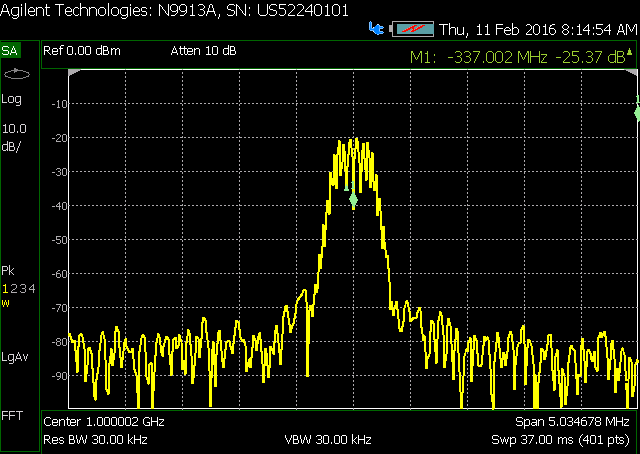
\includegraphics[width=1.0\linewidth]{tx_spec_an}
			\caption{Output of FSK App RF transmit}
			\label{fig:tx_spec_an}
		\end{minipage}
	\end{figure}
\pagebreak
\end{document}
